\documentclass{article}
\usepackage[utf8]{inputenc} % Permite el uso de caracteres del Español
\usepackage[T1]{fontenc}
\usepackage{hyperref}
\usepackage{graphicx}
\usepackage{wrapfig}
\usepackage{subcaption}

% Para ecuaciones
\usepackage{amssymb, amsmath, amsbsy} % simbolitos
\usepackage{upgreek} % para poner letras griegas sin cursiva
\usepackage{cancel} % para tachar
\usepackage{mathdots} % para el comando \iddots
\usepackage{mathrsfs} % para formato de letra
\usepackage{stackrel} % para el comando \stackbin


% set font encoding for PDFLaTeX, XeLaTeX, or LuaTeX
\usepackage{ifxetex,ifluatex}
\newif\ifxetexorluatex
\ifxetex
  \xetexorluatextrue
\else
  \ifluatex
    \xetexorluatextrue
  \else
    \xetexorluatexfalse
  \fi
\fi

\ifxetexorluatex
  \usepackage{fontspec}
\else
  \usepackage[T1]{fontenc}
  \usepackage[utf8]{inputenc}
  \usepackage{lmodern}
\fi

\usepackage{hyperref}

\title{Actividad 9: \\ Sistema de Algebra Computacional Maxima}
\author{Melissa Matrecitos Avila}
\date{28 de Abril de 2018}

% Enable SageTeX to run SageMath code right inside this LaTeX file.
% http://mirrors.ctan.org/macros/latex/contrib/sagetex/sagetexpackage.pdf
% \usepackage{sagetex}

\begin{document}
\maketitle

\section{Introducción}
\begin{wrapfigure} {l}{0.35\textwidth}
  \centering
  \includegraphics[width=0.3\textwidth]{logomax.png}
\end{wrapfigure}
El siguiente reporte corresponde a la actividad 9 del curso de Física Computacional 1, la cual se enfoca a la solución simbólica de ecuaciones, mediante la utilización de software especializado.

Un sistema de álgebra computacional (CAS), es una pieza de software matemático. Permite a un usuario escribir álgebra, cálculo y preguntas estadísticas, usando comandos que son muy parecidos al lenguaje humano, e intenta responder usando la potencia computacional de la computadora.

Una de las CAS más antiguas que existe es una llamada Macsyma. Comenzó su vida de software en 1968 por investigaciones en el MIT. De este se derivaron algunos softwares,  uno de ellos fue Maxim. Esta versión fue abierta en 1999  y continúa desarrollándose como un proyecto de código abierto hasta el día de hoy. En especifico, WxMaxima es la cara bonita de la vieja escuela Maxima CAS. Nos permite escribir texto, hacer informes y, lo que es más importante, tiene menús y botones que nos ayudan a recordar los comandos que necesitamos.

EL reporte presenta un pequeño manual sobre uno de los aspectos básicos de este, la derivación. También se incluye un problema dónde se aplicará lo explicado en el manual. Por último se presentan las secciones de conclusión, bibliografía y apéndice.

\section{Manual}
En esta sección se presenta el manual sobre como derivar utilizando WxMaxima. Primeramente se da una introducción a WxMaxima, como escribir texto explicativo, comando matemáticos, guardar e imprimir. Después se muestra una pequeña introducción a la derivación, también como guardar las salidas en una nueva función, gráfica de derivadas y como obtener valores numéricos.

\subsection{Bases}
\subsubsection{Texto explicativo}
Para escribir texto, agregar un título, una sección, una subsección, etc. tiene dos opciones:
\begin{enumerate}
\item Haciendo uso del menu:

\centerline {Cell $\longrightarrow$ Insert [Text/Heading/etc]}


Y esto colocará un cuadro de texto o cuadro de encabezado en la línea debajo de donde el cursor se ecuentre.

\item Usando Ctrl:

Si escribe cualquier parte de texto, puede hacerlo más ráido con estos accesos directos:
\begin{itemize}
\item Ctrl+1 : Comienza un nuevo cuadro de texto
\item Ctrl+2 : Agrega un título principal
\item Ctrl+3 : Agrega un título de sección
\item Ctrl+4 : Agrega un título de subsección
\item Ctrl+5 : Agrega un título de subsubsección
\end{itemize}
\end{enumerate}
\subsubsection{Comandos matemáticos}

\textbf{Entrada y salida de infromación}: 

Cuando se inicia una sesión, aparecerá la etiqueta "\% i1", que significa entrada 1 (input 1). Se debe escribir un comando válido al lado de esa etiqueta, que termina con un punto y coma y cuando se pulsa la tecla Intro, esa entrada se analizará , simplificado, vinculado a una variable interna "\% i1" y su resultado se mostrará después de una etiqueta "\% o1", que significa salida 1 (output2).

\begin{center}
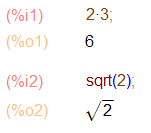
\includegraphics[width=.3\textwidth]{EntradaySalida1.PNG}
\end{center}

Para buscar información de una función o variable especial en el manual, por ejemplo, el registro de funciones que se acaba de utilizar, se usa la función de descripción, que se puede abreviar con un signo de interrogación seguido de espacio y el nombre de la función:

\begin{center}
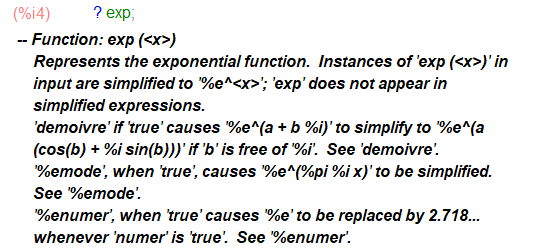
\includegraphics[width=1\textwidth]{Buscar.PNG}
\end{center}

\textbf{Números}:

Maxima acepta números reales y complejos. Los números reales en Maxima pueden ser enteros, racionales, o números de coma flotante (incluso notación científica). Los números irracionales se dejan en esa forma, sin ser aproximados por números de coma flotante, para que en cálculos posteriores la salida coincida con el resultado exacto. Sin embargo que lo que se quiere es una aproximación del número, solo basta en realizar las operaciones en ese formato o bien usar la función "float":

\begin{center}
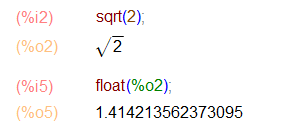
\includegraphics[width=0.5\textwidth]{Float.PNG}
\end{center}

\textbf{Variables}:

Para vincular un objeto a una variable, como un valor numérico, una expresión algebraica o a cualquier otro objeto, se usa el símbolo ":" y no el signo igual "$=$", que se usará para definir ecuaciones matemáticas. El nombre de las variables puede ser cualquier combinación de letras, números y uno de los símbolos $\%$ o $\_$, pero el primer carácter no puede ser un número.
\begin{center}
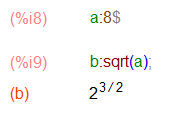
\includegraphics[width=0.3\textwidth]{Variables.PNG}
\end{center}

Otras acciones que se pueden llevar a cabo con variables son: eliminar el valor vinculado a esta con la función "remvalue" y para eliminar todos los valores vinculados a varias variables, se utiliza el comando "remvalue (all)". Otra acción es la de sustituir una variable en una expresión por un valor dado, para lo cual se usa el comando "subst".

\textbf{Lista}:

Una variable también se puede vincular a una lista de valores, como un vector renglón, que se colocan entre corchetes y separados por comas. Por ejemplo, el siguiente comando vincula a "primos" a una lista con los número primos entre el 1 y el 10:

\begin{center}
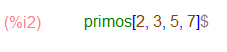
\includegraphics[width=0.3\textwidth]{Lista.PNG}
\end{center}

A las listas se les pueden realizar muchas de las operaciones que se dan entre los números. También a los elementos de una lista se les numera por números enteros que comienzan por 1. Para hacer referencia a un elemento de la lista, se escribe el nombre de la lista y el índice correspondiente se escribe entre corchetes.

Una función muy útil para crear listas es "makelist", que expande una expresión, reemplazando varios valores diferentes para una variable determinada. El primer argumento dado a "makelist" debe ser la expresión a expandir y el segundo argumento es el nombre de la variable que será reemplazada por una secuencia de valores desde un valor inicial hasta un valor máximo definido por el tercer y cuarto argumentos. Si se proporciona un quinto argumento, se usará como el incremento en la secuencia de valores que se reemplazarán; de lo contrario, se usará el incremento predeterminado de 1. Dos ejemplos del uso de esta función son los siguientes:

\begin{center}
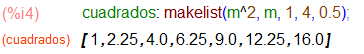
\includegraphics[width=0.5\textwidth]{ListaEjemplo.PNG}
\end{center}
 
\textbf{Constantes}:

Hay algunas constantes matemáticas predefinidas en Maxima. Los nombres de variable vinculados a esas constantes generalmente comienzan con el  símbolo $\%$. Tres constantes importantes son el número $\pi$ , vinculado a $\%$ pi, el número de Euler $e$, la base de los logaritmos naturales, vinculado a $\% e$ y el número imaginario $i$, vinculado a $\%$ i.

\begin{center}
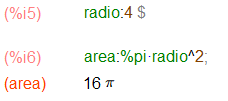
\includegraphics[width=0.4\textwidth]{Constantes.PNG}
\end{center}

\subsubsection{Guardar trabajo}
Para guardar el trabajo realizado se tienen dos opciones:

\begin{enumerate}
\item Haciendo uso del menu:

\centerline {File $\longrightarrow$ Save}
\centerline {File $\longrightarrow$ Save As}

\item Usando Ctrl:

\centerline {Ctrl+s: Save}
\centerline {Ctrl+Shift+s: Save As}
\end{enumerate}

\subsection{Introducción a la derivada}

El comando para calcular la derivada de cualquier expresión en Maxima es \textbf{diff ()}, la cual tiene se utiliza utilizando la siguiente forma:

\centerline {diff (expresión, variable, [orden de derivada (solo si es mayor que 1)])}

\begin{center}
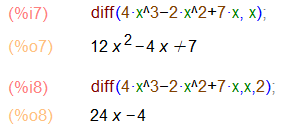
\includegraphics[width=0.4\textwidth]{Derivada1.PNG}
\end{center}

Otra manera de encontrar la derivada de un función, es definiendo esta y aplicando el comando anterior de la siguiente manera: 

\begin{center}
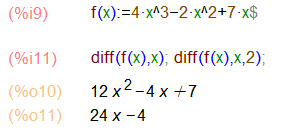
\includegraphics[width=0.4\textwidth]{Derivada2.PNG}
\end{center}

\subsection{Guardando la salida en una nueva función}

Hay veces en las que es necesario tener a la mano la derivada de una función, ya sea para saber cuando ésta es cero o simplemente calcular su valor. Para eso es necesario guardar el valor de la derivada en una nueva función, esto se logra de la siguiente manera:

\begin{center}
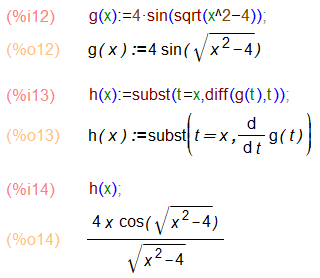
\includegraphics[width=0.4\textwidth]{Funcionderivada.PNG}
\end{center}

Es decir, diferenciamos f (t) con respecto a t, y luego remplazamos a t por x. Esto es para que a momento de querer un valor de la derivada, no haya problema con los argumentos de las funciones. Así si queremos encontrar la derivada evaluada en algún punto:

\begin{center}
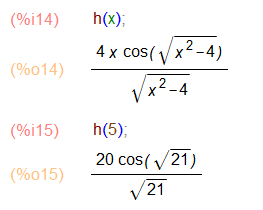
\includegraphics[width=0.4\textwidth]{Funcionderivada2.PNG}
\end{center}

\subsection{Graficando derivadas}

Ya que se pueden guardar las derivadas en nuevas funciones, se puede hacer con ellas todo lo que se puede hacer con cualquier función, tal como ser graficadas, por ejemplo:

\begin{center}
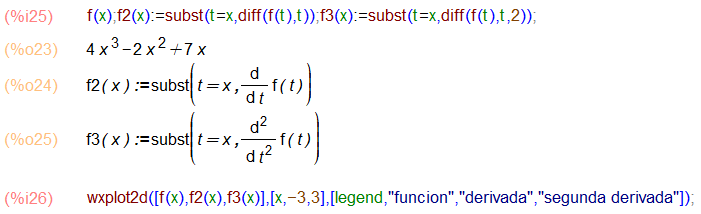
\includegraphics[width=0.8\textwidth]{Graficaderivadas.PNG}
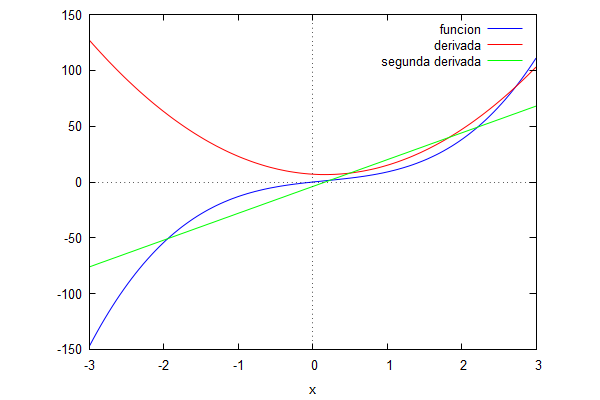
\includegraphics[width=0.7\textwidth]{Graficaderivadas2.PNG}
\end{center}

\subsubsection{Racionalizando el proceso de sustitución}

Para evitar tener que realizar el procedimiento de diferencias y sustituir varias veces, se puede crear una función que realice todos esos pasos por nosotros, tal como se muestra a continuación:

\begin{center}
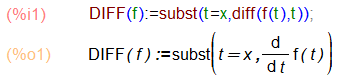
\includegraphics[width=0.4\textwidth]{Derivadautomatica.PNG}
\end{center}

Lo que se hizo fue una nueva operación (llamada DIFF ()) que toma una función f(x) y realiza el proceso de diferenciación y sustitución con esta. A continuación un ejemplo de como se utiliza:

\begin{center}
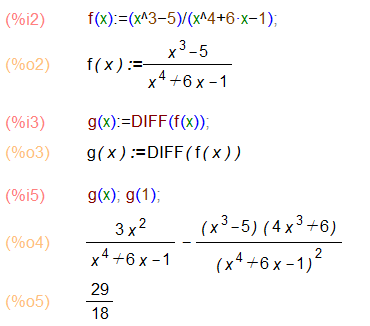
\includegraphics[width=0.4\textwidth]{EjemDerivadautomatica.PNG}
\end{center}

Esta función se puede generalizar para calcular derivadas de orden mayor, solo que será necesario especificar el orden de la derivada:

\begin{center}
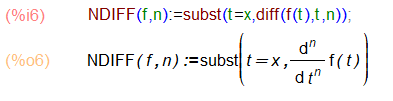
\includegraphics[width=0.4\textwidth]{Derivadautomatica2.PNG}
\end{center}

Con estas nuevas funciones, el proceso de graficar las derivadas se simplifica muchísimo, permitiéndonos hacer ejercicios como el siguiente:

\begin{center}
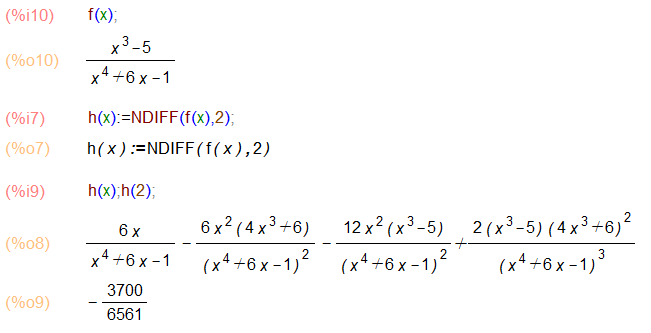
\includegraphics[width=0.7\textwidth]{EjemDerivadautomatica2.PNG}
\end{center}

\subsubsection{Una forma aún más simplificada de obtener derivados de orden superior}

Una forma diferente de obtener derivados de orden superior se basa en la creación de una lista vacía, dónde, en el termino 0 se se escribe a función a diferenciar, después, se define el elemento n de la lista como la derivada del elemento n-1;

\begin{center}
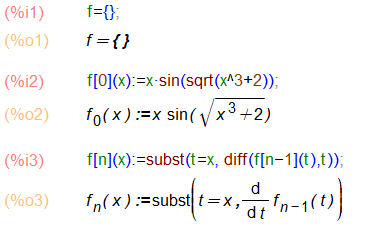
\includegraphics[width=.5\textwidth]{DerivadaenLista.PNG}
\end{center}

Un ejemplo de esto es:

\begin{center}
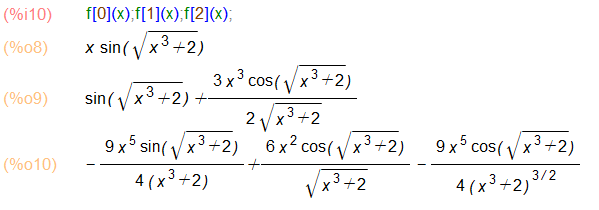
\includegraphics[width=.8\textwidth]{DerivadaenLista2.PNG}
\end{center}

\subsection{Obteniendo valores numéricos}

Si se desea obtener una aproximación a una derivada, lo único que se debe de hacer es utilizar el comando float a la evaluación de la derivada, tal como se muestra a continuación:

\begin{center}
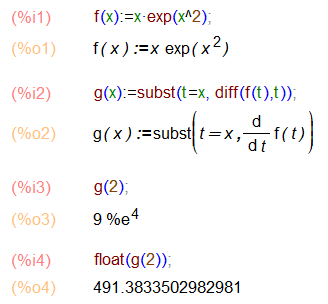
\includegraphics[width=.5\textwidth]{Numerica.PNG}
\end{center}

Sin embargo, si solo va a pedir un valor de la derivada, entonces es más rápido simplemente sustituirlo directamente como un valor flotante, en el siguiente ejemplo se muestra una comparación de un numero exacto y uno flotante:

\begin{center}
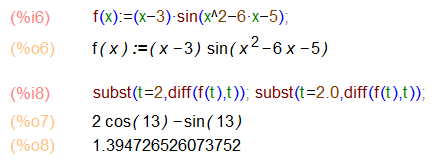
\includegraphics[width=.5\textwidth]{Numerica2.PNG}
\end{center}

O bien, si se va a solicitar una gran cantidad de salidas en modo flotante de una misma función, simplemente se forza el comando float () en la definición:

\begin{center}
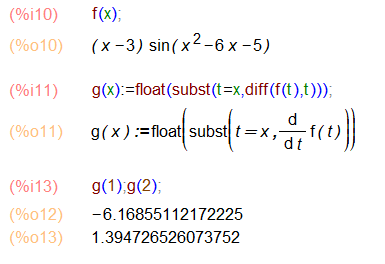
\includegraphics[width=.5\textwidth]{Numerica3.PNG}
\end{center}

\section{Problema de Aplicación}
\begin{wrapfigure} {r}{0.35\textwidth}
  \centering
  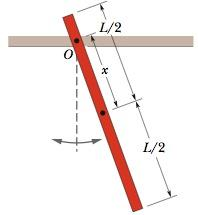
\includegraphics[width=0.3\textwidth]{Pendulo.jpg}
\end{wrapfigure}
Se forma un péndulo físico por medio de una barra de L=0.5m, de masa m=0.8 kg pivotada a una distancia x=0.18 m medida desde su centro de masa. Encontrar:
\begin{enumerate}
    \item El periodo para pequeñas oscilaciones.
    \item La distancia x, tal que el periodo sea mínimo
\end{enumerate}

Del problema tenemos que:

\begin{center}
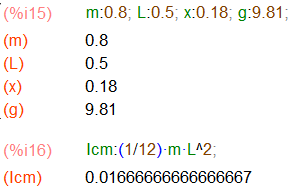
\includegraphics[width=.5\textwidth]{Pdatos.PNG}
\end{center}

Entonces para el inciso 1, sustituimos los datos en la ecuación para el periodo y obtenemos:
\begin{center}
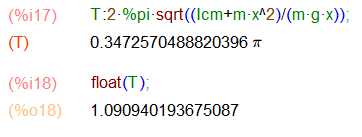
\includegraphics[width=.5\textwidth]{Pperiodo.PNG}
\end{center}

Para el inciso 2, definimos la función del periodo y realizamos su gráfica, para observar su comportamiento:

\begin{center}
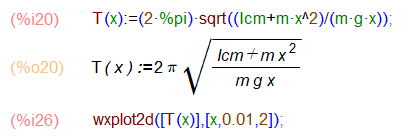
\includegraphics[width=.5\textwidth]{Pfuncion.PNG}
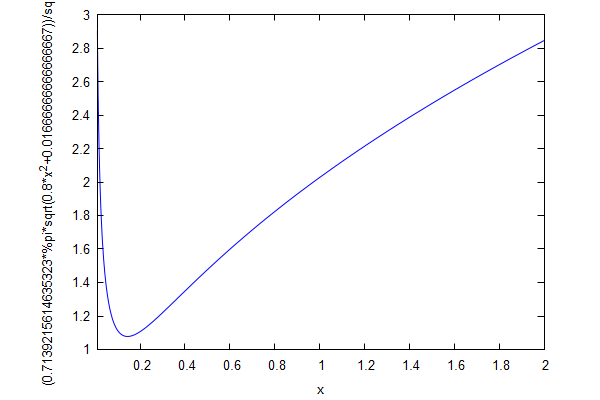
\includegraphics[width=.5\textwidth]{Pgrafica.png}
\end{center}

Se obtienen la primera y segunda derivada de la función:
\begin{center}
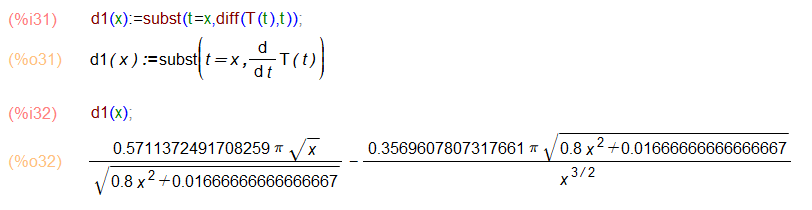
\includegraphics[width=.8\textwidth]{Pderivada.PNG}
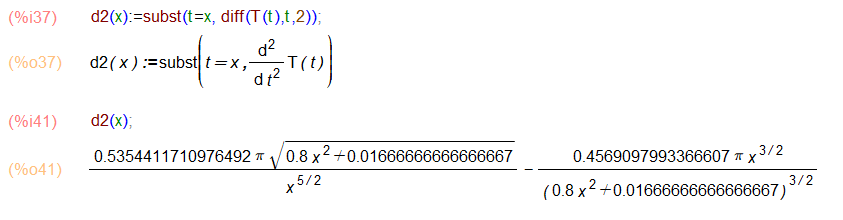
\includegraphics[width=.8\textwidth]{Pderivada2.PNG}
\end{center}

Después se encuentra la raíz de la primera derivada y se evalua en la primera y segunda derivada para verificar que sea mínimo:
\begin{center}
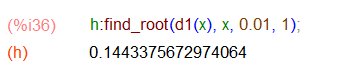
\includegraphics[width=.5\textwidth]{Praiz.PNG}
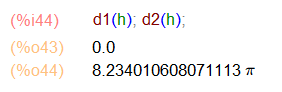
\includegraphics[width=.5\textwidth]{Presultado.PNG}
\end{center}
Cómo la primera derivada es igual a cero y la segunda es un númerpositivo, entonces con x=0.144 m se obtendrá un periodo mínimo.
\section{Conclusión}
Consideró que ha sido una de las mejores actividades del curso, ya que se ve directamente la aplicación del los CAS a los problemas con los que me enfrentó en mis demás materias. Además realizar yo este manual me permitió entender más a fondo como utilizar WxMaxima, llegando a formar parte de una de las herramientas que seguramente utilizare durante la carrera.

\section{Bibliografía}
\begin{itemize}
\item A. Maxima Tutorial. (2018). Def.fe.up.pt. Recuperado el 28 de Abril de 2018, de \url{https://def.fe.up.pt/dynamics/maxima_tutorial.html}
\item wxMaxima Tutorials. (2018). Scotchildress.com. Recuperado el 28 de Abril de 2018, de \url{http://www.scotchildress.com/wxmaxima/}
\item Logo de Maxima: \url{https://commons.wikimedia.org/wiki/File:Maxima-new.svg}
\end{itemize}
\section{Apéndice}
\begin{enumerate}
\item ¿Cuál fue tu primera impresión de wxmaxima?

Me gustó muchísimo, ya que es muy fácil de utilizar, sobre todo por el lenguaje de los comandos y como expresa el resultado.
\item ¿Crees que esta herramienta puede ser útil en otros de tus cursos?

Sí, por que simplifica mucho el trabajo, además de que puedes comparar si los resultados que obtuviste son los correctos.
\item ¿Qué se te dificultó mas en esta actividad?

Nada, me pareció una actividad muy sencilla.
\item ¿Se te hizo compleja esta actividad? ¿Cómo la mejorarías? 

No, así como está me parece muy bien.
\end{enumerate}
\end{document}
